
\documentclass[10pt]{article}
\usepackage[utf8]{inputenc}

\title{Estatística e Probabilidade para Computação}
\author{Ana Letícia da Costa Saraiva}
\date{November 2019}

\usepackage{natbib}
\usepackage{graphicx}

\begin{document}

\maketitle

\section{Introdução}
A disciplina Estatística e Probabilidade para Computação compreende áreas do conhecimento como análise de dados e cálculo de possibilidades, muito utilizadas em diversos campos da matemática e computação. Na cadeira, alunos aprendem a base para analisar padrões de dados e fórmulas para calcular tais probabilidades em suas várias formas, entre elas a demonstrada pela Distribuição de Poisson.\cite{sitedisciplina}

\begin{figure}[h!]
\centering
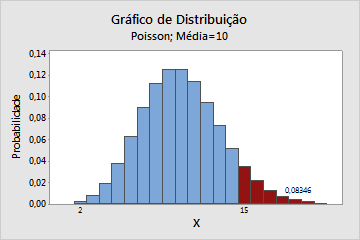
\includegraphics[scale=0.9]{distribuicao_poisson.png}
\caption{Distribuição de Poisson em probabilidade. \citep{grafico}}
\label{fig:Análise de Dados}
\end{figure}

\section{Relevância}
A compreensão de análise de dados na disciplina se mostra principalmente importante na computação dentro das áreas de Data Science e Machine Learning, pois essas utilizam de predições e reconhecimento de padrões para resolução de problemas através de dados acumulados.\cite{ML}


\section{Relação com outras disciplinas}
A cadeira exige apenas a disciplina de Cálculo I como pré-requisito. As cadeiras relacionadas incluem as eletivas IF702 - Redes Neurais e IF706 - Tópicos Avançados em Inteligência Artificial .
\cite{siteeletivas}
\bibliographystyle{plain}
\bibliography{alcs.bib}
\end{document}
